% Options for packages loaded elsewhere
\PassOptionsToPackage{unicode}{hyperref}
\PassOptionsToPackage{hyphens}{url}
%
\documentclass[
]{article}
\usepackage{lmodern}
\usepackage{amssymb,amsmath}
\usepackage{ifxetex,ifluatex}
\ifnum 0\ifxetex 1\fi\ifluatex 1\fi=0 % if pdftex
  \usepackage[T1]{fontenc}
  \usepackage[utf8]{inputenc}
  \usepackage{textcomp} % provide euro and other symbols
\else % if luatex or xetex
  \usepackage{unicode-math}
  \defaultfontfeatures{Scale=MatchLowercase}
  \defaultfontfeatures[\rmfamily]{Ligatures=TeX,Scale=1}
\fi
% Use upquote if available, for straight quotes in verbatim environments
\IfFileExists{upquote.sty}{\usepackage{upquote}}{}
\IfFileExists{microtype.sty}{% use microtype if available
  \usepackage[]{microtype}
  \UseMicrotypeSet[protrusion]{basicmath} % disable protrusion for tt fonts
}{}
\makeatletter
\@ifundefined{KOMAClassName}{% if non-KOMA class
  \IfFileExists{parskip.sty}{%
    \usepackage{parskip}
  }{% else
    \setlength{\parindent}{0pt}
    \setlength{\parskip}{6pt plus 2pt minus 1pt}}
}{% if KOMA class
  \KOMAoptions{parskip=half}}
\makeatother
\usepackage{xcolor}
\IfFileExists{xurl.sty}{\usepackage{xurl}}{} % add URL line breaks if available
\IfFileExists{bookmark.sty}{\usepackage{bookmark}}{\usepackage{hyperref}}
\hypersetup{
  pdftitle={Tarea 2: Modelos lineales generalizados y no paramétricos},
  pdfauthor={Angie Rodríguez Duque \& César Saavedra Vanegas},
  hidelinks,
  pdfcreator={LaTeX via pandoc}}
\urlstyle{same} % disable monospaced font for URLs
\usepackage[margin=1in]{geometry}
\usepackage{color}
\usepackage{fancyvrb}
\newcommand{\VerbBar}{|}
\newcommand{\VERB}{\Verb[commandchars=\\\{\}]}
\DefineVerbatimEnvironment{Highlighting}{Verbatim}{commandchars=\\\{\}}
% Add ',fontsize=\small' for more characters per line
\usepackage{framed}
\definecolor{shadecolor}{RGB}{248,248,248}
\newenvironment{Shaded}{\begin{snugshade}}{\end{snugshade}}
\newcommand{\AlertTok}[1]{\textcolor[rgb]{0.94,0.16,0.16}{#1}}
\newcommand{\AnnotationTok}[1]{\textcolor[rgb]{0.56,0.35,0.01}{\textbf{\textit{#1}}}}
\newcommand{\AttributeTok}[1]{\textcolor[rgb]{0.77,0.63,0.00}{#1}}
\newcommand{\BaseNTok}[1]{\textcolor[rgb]{0.00,0.00,0.81}{#1}}
\newcommand{\BuiltInTok}[1]{#1}
\newcommand{\CharTok}[1]{\textcolor[rgb]{0.31,0.60,0.02}{#1}}
\newcommand{\CommentTok}[1]{\textcolor[rgb]{0.56,0.35,0.01}{\textit{#1}}}
\newcommand{\CommentVarTok}[1]{\textcolor[rgb]{0.56,0.35,0.01}{\textbf{\textit{#1}}}}
\newcommand{\ConstantTok}[1]{\textcolor[rgb]{0.00,0.00,0.00}{#1}}
\newcommand{\ControlFlowTok}[1]{\textcolor[rgb]{0.13,0.29,0.53}{\textbf{#1}}}
\newcommand{\DataTypeTok}[1]{\textcolor[rgb]{0.13,0.29,0.53}{#1}}
\newcommand{\DecValTok}[1]{\textcolor[rgb]{0.00,0.00,0.81}{#1}}
\newcommand{\DocumentationTok}[1]{\textcolor[rgb]{0.56,0.35,0.01}{\textbf{\textit{#1}}}}
\newcommand{\ErrorTok}[1]{\textcolor[rgb]{0.64,0.00,0.00}{\textbf{#1}}}
\newcommand{\ExtensionTok}[1]{#1}
\newcommand{\FloatTok}[1]{\textcolor[rgb]{0.00,0.00,0.81}{#1}}
\newcommand{\FunctionTok}[1]{\textcolor[rgb]{0.00,0.00,0.00}{#1}}
\newcommand{\ImportTok}[1]{#1}
\newcommand{\InformationTok}[1]{\textcolor[rgb]{0.56,0.35,0.01}{\textbf{\textit{#1}}}}
\newcommand{\KeywordTok}[1]{\textcolor[rgb]{0.13,0.29,0.53}{\textbf{#1}}}
\newcommand{\NormalTok}[1]{#1}
\newcommand{\OperatorTok}[1]{\textcolor[rgb]{0.81,0.36,0.00}{\textbf{#1}}}
\newcommand{\OtherTok}[1]{\textcolor[rgb]{0.56,0.35,0.01}{#1}}
\newcommand{\PreprocessorTok}[1]{\textcolor[rgb]{0.56,0.35,0.01}{\textit{#1}}}
\newcommand{\RegionMarkerTok}[1]{#1}
\newcommand{\SpecialCharTok}[1]{\textcolor[rgb]{0.00,0.00,0.00}{#1}}
\newcommand{\SpecialStringTok}[1]{\textcolor[rgb]{0.31,0.60,0.02}{#1}}
\newcommand{\StringTok}[1]{\textcolor[rgb]{0.31,0.60,0.02}{#1}}
\newcommand{\VariableTok}[1]{\textcolor[rgb]{0.00,0.00,0.00}{#1}}
\newcommand{\VerbatimStringTok}[1]{\textcolor[rgb]{0.31,0.60,0.02}{#1}}
\newcommand{\WarningTok}[1]{\textcolor[rgb]{0.56,0.35,0.01}{\textbf{\textit{#1}}}}
\usepackage{longtable,booktabs}
% Correct order of tables after \paragraph or \subparagraph
\usepackage{etoolbox}
\makeatletter
\patchcmd\longtable{\par}{\if@noskipsec\mbox{}\fi\par}{}{}
\makeatother
% Allow footnotes in longtable head/foot
\IfFileExists{footnotehyper.sty}{\usepackage{footnotehyper}}{\usepackage{footnote}}
\makesavenoteenv{longtable}
\usepackage{graphicx,grffile}
\makeatletter
\def\maxwidth{\ifdim\Gin@nat@width>\linewidth\linewidth\else\Gin@nat@width\fi}
\def\maxheight{\ifdim\Gin@nat@height>\textheight\textheight\else\Gin@nat@height\fi}
\makeatother
% Scale images if necessary, so that they will not overflow the page
% margins by default, and it is still possible to overwrite the defaults
% using explicit options in \includegraphics[width, height, ...]{}
\setkeys{Gin}{width=\maxwidth,height=\maxheight,keepaspectratio}
% Set default figure placement to htbp
\makeatletter
\def\fps@figure{htbp}
\makeatother
\setlength{\emergencystretch}{3em} % prevent overfull lines
\providecommand{\tightlist}{%
  \setlength{\itemsep}{0pt}\setlength{\parskip}{0pt}}
\setcounter{secnumdepth}{-\maxdimen} % remove section numbering

\title{Tarea 2: Modelos lineales generalizados y no paramétricos}
\author{Angie Rodríguez Duque \& César Saavedra Vanegas}
\date{Octubre 22 de 2020}

\begin{document}
\maketitle

\hypertarget{actividad-1}{%
\section{Actividad 1}\label{actividad-1}}

Se dispone de los tiempos de vida (tiempos hasta que fallan, en horas)
de \(49\) recipientes de presión sometidos a un nivel de carga del
\(70\%\). De esta manera, se considera el problema de los recipientes de
presión, cuya duración, se presume, sigue una distribución de Weibull.

\hypertarget{distribuciuxf3n-weibull}{%
\subsubsection{Distribución Weibull}\label{distribuciuxf3n-weibull}}

Para estudiar la variable ``Tiempos de falla (Horas)'' se procede a
utilizar la distribución de Weibull, cuya función de densidad es:

\[f(y;\lambda,\theta)=\displaystyle\frac{\lambda y^{\lambda-1}}{\theta^{\lambda}}exp \left[-\left(\frac{y}{\theta}\right)^{\lambda}\right]\]

\hypertarget{transformaciuxf3n}{%
\subsubsection{Transformación}\label{transformaciuxf3n}}

Se realiza el cambio de las unidades de la variable de respuesta, la
cual está reportada originalmente en horas. En esta ocasión se decide
trabajar con el ``Tiempo de falla'' en días.

\[1 día\longrightarrow 24 horas\]

Posteriormente, se lleva a cabo la elección de una muestra al azar de
\(36\) recipientes y se estima \(\theta\) por el método de
Newton-Raphson.

Como asumimos que conocemos \(\lambda\), la solución de \(U=0\) será el
estimador \(\hat{\theta}\) del parámetro de escala \(\theta\). En este
caso, se decidió trabajar con 5 valores para lambda, esto es, \(1\),
\(1.5\), \(2\), \(2.5\) y \(3\)

\hypertarget{el-muxe9todo-de-newton-raphson}{%
\subsubsection{El método de
Newton-Raphson}\label{el-muxe9todo-de-newton-raphson}}

Se propone explorar este problema de estimación usando el método de
Newton-Raphson, el cual es un algoritmo basado en la derivada que
permite encontrar aproximaciones de los ceros o raíces de una función
real derivable. En este caso particular se hará uso de la función U de
scoring para la Weibull y se asumirá \(\lambda\) conocido y \(U\) será
el estimador \(\hat{\theta}\) del parámetro de escala \(\theta\). La
descripción del método es la siguiente:

\begin{enumerate}
\def\labelenumi{\arabic{enumi}.}
\item
  Se elige \(x_{0}\) en el eje de las \(x\), asumiendo que está cerca de
  la solución de \(f(x)=0\) (raíz buscada)
\item
  Calculamos la ecuación punto pendiente de la recta tangente de la
  función en \((x_{0},f(x_{0}))\), a saber
  \(y-f(x_{0})=f’(x_{0})(x-x_{0})\) (1).
\item
  Esta recta debe intersecar al eje de las x, en un punto más cercano a
  la raíz buscada; en el punto \((x_{1},0)\).
\item
  El punto \((x_{1},0)\) satisface la ecuación (1) y sustituyendo queda:
\end{enumerate}

\[0-f(x_{0})=f’(x_{0})(x-x_{0}) \hspace{2cm} (2)\]

\begin{enumerate}
\def\labelenumi{\arabic{enumi}.}
\setcounter{enumi}{4}
\tightlist
\item
  Si \(f’(x_{0})\neq0\), entonces despejando \(x_{i}\) en (2) se
  obtiene:
\end{enumerate}

\[x_{1}=x_{0}-\frac{f(x_{0})}{f’(x_{0})}\]

\begin{enumerate}
\def\labelenumi{\arabic{enumi}.}
\setcounter{enumi}{5}
\tightlist
\item
  Repetimos el procedimiento anterior para \(x_{0}\), pero ahora
  comenzando en \(x_{1}\), en cuyo caso se obtiene:
\end{enumerate}

\[x_{2}=x_{1}-\frac{f(x_{0})}{f’(x_{0})}\]

De forma que \(x_{2}\) está más cerca de la raíz buscada que \(x_{1}\).

\begin{enumerate}
\def\labelenumi{\arabic{enumi}.}
\setcounter{enumi}{6}
\tightlist
\item
  Iterando cada vez con el número obtenido, se construye una secuencia:
  \(x_{0},x_{1},x_{2},..., x_{n}\) de números cada vez más próximos a la
  raíz tales que:
\end{enumerate}

\[x_{n+1}=x_{n}-\frac{f(x_{0})}{f’(x_{0})} \hspace{2cm} (3)\] De acuerdo
con los pasos enumerados anteriormente se obtienen los siguientes
resultados en los que se usó como valor inicial el promedio de los datos
\(\bar{y}=388.5787\):

\begin{longtable}[]{@{}llllll@{}}
\toprule
Interacción & \(\lambda=1\) & \(\lambda=1.5\) & \(\lambda=2\) &
\(\lambda=2.5\) & \(\lambda=3\)\tabularnewline
\midrule
\endhead
1 & 388.5787 & 388.5787 & 388.5787 & 388.5787 & 388.5787\tabularnewline
2 & & 408.2362 & 420.6631 & 428.5779 & 433.5102\tabularnewline
3 & & 410.7335 & 428.6631 & 443.3022 & 454.9522\tabularnewline
4 & & 410.7684 & 429.1123 & 444.8338 & 458.7434\tabularnewline
5 & & 410.7684 & 429.1133 & 444.8485 & 458.7434\tabularnewline
6 & & & 429.1133 & 444.8485 & 458.7434\tabularnewline
\bottomrule
\end{longtable}

A partir de la tabla anterior, se observa que la primera iteración para
los diferentes lambdas corresponde a la media de los tiempos de falla en
días, el cual es el valor incial definido en el algoritmo. También es
posible evidenciar que en el caso de \(\lambda=1\) se obtiene tan solo 1
iteración, mientras que para \(\lambda=1.5\) se obtienen 5 iteraciones,
y para \(\lambda=2\), \(2.5\) y \(3\) el número de iteraciones es el
mismo, esto es, 6. Para cada uno de estos casos el valor estimado del
parámetro \(\theta\) resulta ser mayor a medida que se incrementa el
parámetro de pertubación lambda.

\hypertarget{actividad-2}{%
\section{Actividad 2}\label{actividad-2}}

\hypertarget{base-de-datos}{%
\subsubsection{Base de datos}\label{base-de-datos}}

\begin{Shaded}
\begin{Highlighting}[]
\KeywordTok{dim}\NormalTok{(Datos)}
\end{Highlighting}
\end{Shaded}

\begin{verbatim}
## [1] 1599   12
\end{verbatim}

Este conjunto de datos de vino tinto consta de 1599 observaciones y 12
variables, 11 de las cuales son sustancias químicas. Las variables son:

\begin{enumerate}
\def\labelenumi{\arabic{enumi}.}
\item
  \textbf{Acidez fija:} La mayoría de los ácidos implicados en el vino
  son fijos o no volátiles (no se evaporan fácilmente).
\item
  \textbf{Acidez volátil:} La cantidad de ácido acético en el vino, que
  en niveles demasiado altos puede provocar un sabor desagradable a
  vinagre.
\item
  \textbf{Ácido cítrico:} Encontrado en pequeñas cantidades, el ácido
  cítrico puede agregar ``frescura'' y sabor a los vinos.
\item
  \textbf{Azúcar residual:} Es la cantidad de azúcar que queda después
  de que se detiene la fermentación, es raro encontrar vinos con menos
  de 1 gramo / litro y los vinos con más de 45 gramos / litro se
  consideran dulces.
\item
  \textbf{Cloruros:} Es la cantidad de sal del vino.
\item
  \textbf{Dióxido de azufre libre:} La forma libre de \(SO_{2}\) existe
  en equilibrio entre el \(SO_{2}\) molecular (como gas disuelto) y el
  ion bisulfito; Previene el crecimiento microbiano y la oxidación del
  vino.
\item
  \textbf{Dióxido de azufre total:} Es la cantidad de formas libres y
  unidas de \(SO_{2}\); en concentraciones bajas, el \(SO_{2}\) es
  mayormente indetectable en el vino, pero en concentraciones de
  \(SO_{2}\) libre superiores a 50 ppm, el \(SO_{2}\) se hace evidente
  en la nariz y el sabor del vino.
\item
  \textbf{Densidad:} La densidad es cercana a la del agua dependiendo
  del porcentaje de alcohol y contenido de azúcar.
\item
  \textbf{pH:} Describe qué tan ácido o básico es un vino en una escala
  de 0 (muy ácido) a 14 (muy básico); la mayoría de los vinos están
  entre 3-4 en la escala de pH.
\item
  \textbf{Sulfatos:} Aditivo del vino que puede contribuir a los niveles
  de dióxido de azufre \((SO_{2})\), que actúa como antimicrobiano y
  antioxidante.
\item
  \textbf{Alcohol:} El porcentaje de contenido de alcohol del vino.
\item
  \textbf{Calidad:} Variable de respuesta (basada en datos sensoriales,
  puntuación entre 0 y 10).
\end{enumerate}

\hypertarget{estaduxedsticas-descriptivas}{%
\subsubsection{Estadísticas
descriptivas}\label{estaduxedsticas-descriptivas}}

\begin{Shaded}
\begin{Highlighting}[]
\KeywordTok{summary}\NormalTok{(Datos)}
\end{Highlighting}
\end{Shaded}

\begin{verbatim}
##  fixed.acidity   volatile.acidity  citric.acid    residual.sugar  
##  Min.   : 4.60   Min.   :0.1200   Min.   :0.000   Min.   : 0.900  
##  1st Qu.: 7.10   1st Qu.:0.3900   1st Qu.:0.090   1st Qu.: 1.900  
##  Median : 7.90   Median :0.5200   Median :0.260   Median : 2.200  
##  Mean   : 8.32   Mean   :0.5278   Mean   :0.271   Mean   : 2.539  
##  3rd Qu.: 9.20   3rd Qu.:0.6400   3rd Qu.:0.420   3rd Qu.: 2.600  
##  Max.   :15.90   Max.   :1.5800   Max.   :1.000   Max.   :15.500  
##    chlorides       free.sulfur.dioxide total.sulfur.dioxide    density      
##  Min.   :0.01200   Min.   : 1.00       Min.   :  6.00       Min.   :0.9901  
##  1st Qu.:0.07000   1st Qu.: 7.00       1st Qu.: 22.00       1st Qu.:0.9956  
##  Median :0.07900   Median :14.00       Median : 38.00       Median :0.9968  
##  Mean   :0.08747   Mean   :15.87       Mean   : 46.47       Mean   :0.9967  
##  3rd Qu.:0.09000   3rd Qu.:21.00       3rd Qu.: 62.00       3rd Qu.:0.9978  
##  Max.   :0.61100   Max.   :72.00       Max.   :289.00       Max.   :1.0037  
##        pH          sulphates         alcohol         quality     
##  Min.   :2.740   Min.   :0.3300   Min.   : 8.40   Min.   :3.000  
##  1st Qu.:3.210   1st Qu.:0.5500   1st Qu.: 9.50   1st Qu.:5.000  
##  Median :3.310   Median :0.6200   Median :10.20   Median :6.000  
##  Mean   :3.311   Mean   :0.6581   Mean   :10.42   Mean   :5.636  
##  3rd Qu.:3.400   3rd Qu.:0.7300   3rd Qu.:11.10   3rd Qu.:6.000  
##  Max.   :4.010   Max.   :2.0000   Max.   :14.90   Max.   :8.000
\end{verbatim}

\begin{figure}
\centering
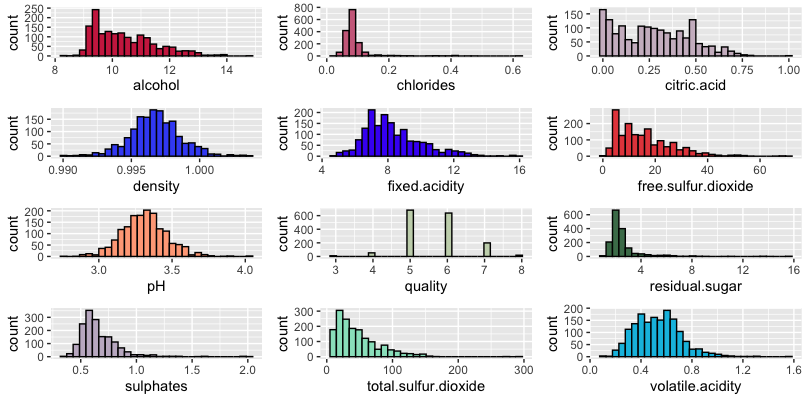
\includegraphics[width=6.77083in,height=\textheight]{G1.png}
\caption{Distribución de las variables}
\end{figure}

\hypertarget{observaciones}{%
\subsubsection{Observaciones:}\label{observaciones}}

\begin{itemize}
\item
  Algunas de las variables tienen distribuciones normales (densidad,
  acidez fija, pH, acidez volátil).
\item
  Algunas variables están un poco sesgadas hacia el extremo inferior de
  los valores (cloruros, ácido cítrico, azúcar residual, dióxido de
  azufre total).
\item
  La variable calidad tiene solo 6 valores discretos.
\end{itemize}

\begin{Shaded}
\begin{Highlighting}[]
\KeywordTok{corrplot}\NormalTok{(}\KeywordTok{cor}\NormalTok{(Datos), }\DataTypeTok{method=}\StringTok{"square"}\NormalTok{, }\DataTypeTok{type=}\StringTok{"upper"}\NormalTok{, }\DataTypeTok{order=}\StringTok{"hclust"}\NormalTok{, }\DataTypeTok{tl.col=}\StringTok{"black"}\NormalTok{)}
\end{Highlighting}
\end{Shaded}

\begin{center}\includegraphics{Informe_files/figure-latex/unnamed-chunk-5-1} \end{center}

\begin{itemize}
\item
  La densidad tiene una correlación muy fuerte con la acidez fija.
\item
  Las variables más fuertemente correlacionadas con la calidad son la
  acidez volátil y el alcohol.
\item
  El alcohol tiene una correlación negativa con la densidad. Esto es
  evidente por el hecho de que la densidad del agua es mayor que la
  densidad del alcohol.
\item
  Es posible observar que las variables pH y acidez fija presentan una
  correlación negativamente fuerte, lo cual nos indica que a mayor pH
  menor será la acidez, y viceversa, a menor pH mayor acidez. Lo cual se
  ve reflejado en la calidad final del vino.
\end{itemize}

\hypertarget{variable-indicadora-phi}{%
\subsubsection{Variable indicadora: pHi}\label{variable-indicadora-phi}}

Se convierte la variable ``pH'' en una variable indicadora con tres
niveles: ``alto'', ``medio'' y ``bajo'', esta nueva variable se
denomina: ``pHi''. Para dicha transformación se realiza el siguiente
procedimiento:

\[Rango=\displaystyle\frac{Máx(pH)-Mín(pH)}{3}\]
\[Rango=\displaystyle\frac{4.01-2.74}{3}=0.4233333\] De esta manera, los
límites de cada intervalo son:

\begin{itemize}
\tightlist
\item
  \(a = mín(pH)=2.74\)
\item
  \(b = a + Rango=3.163333\)
\item
  \(c = b + Rango=3.586667\)
\item
  \(d = c + Rango=4.01\)
\end{itemize}

\begin{longtable}[]{@{}lrll@{}}
\toprule
Nivel & Criterio & Intervalo & Conteo\tabularnewline
\midrule
\endhead
Bajo & pH\textless b & \([2.74;3.163333)\) & 267\tabularnewline
Medio & pH \(\geq\) b \& pH\textless c & \([3.163333;3.586667)\) &
1269\tabularnewline
Alto & pH \(\geq\) c & \([3.586667;4.01)\) & 63\tabularnewline
\bottomrule
\end{longtable}

A partir de la siguiente figura es posible observar como el nivel de
\(pH\) con mayor frecuencia es aquel que se denomina como ``medio'' con
1269 observaciones, mientras que los niveles ``bajo'' y ``alto'',
presentan frecuencias muy bajas, esto es, 267 y 63 respectivamente.

\begin{Shaded}
\begin{Highlighting}[]
\NormalTok{G2}
\end{Highlighting}
\end{Shaded}

\begin{center}\includegraphics{Informe_files/figure-latex/unnamed-chunk-8-1} \end{center}

Partiendo de lo anterior también se hace importante conocer el
comportamiento de las dos variables de predicción, Acidez fija y pH,
teniendo en cuenta las categorías (bajo, medio, alto) definidas a partir
de los valores de pH para conocer cual es el comportamiento de estas, su
posible relación y como podrían afectar la predicción de la calidad del
vino en el modelo que se desea estudiar.

\begin{Shaded}
\begin{Highlighting}[]
\NormalTok{G3}
\end{Highlighting}
\end{Shaded}

\begin{center}\includegraphics{Informe_files/figure-latex/unnamed-chunk-10-1} \end{center}

Este figura presenta un comportamiento decreciente y se complementa con
el gráfico de correlaciones presentado anteriormente en el cual era
posible observar que las variables pH y acidez fija presentaban una
correlación negativamente fuerte, lo cual nos indica que a mayor pH
menor será la acidez. Esto podría verse reflejado en el modelo que se
desea plantear y en si estas variables resultan ser o no significativas
en la explicación de la calidad del vino.

\hypertarget{modelo-con-variable-indicadora-phi}{%
\subsubsection{Modelo con variable indicadora
pHi}\label{modelo-con-variable-indicadora-phi}}

En esta sección, se procede a generar un modelo logístico con variable
de respuesta ordinal, ya que la variable de respuesta ``calidad'' tiene
una jerarquía, esto es, una puntuación entre 0 y 10, donde 0 representa
una mala calidad y 10 una calidad de vino excelente.

\begin{Shaded}
\begin{Highlighting}[]
\NormalTok{fit =}\StringTok{ }\KeywordTok{vglm}\NormalTok{(quality }\OperatorTok{~}\StringTok{ }\NormalTok{fixed.acidity }\OperatorTok{+}\StringTok{ }\NormalTok{pHi, }\DataTypeTok{data =}\NormalTok{ Datos, }\DataTypeTok{family =} \KeywordTok{cumulative}\NormalTok{(}\DataTypeTok{parallel =} \OtherTok{TRUE}\NormalTok{))}
\end{Highlighting}
\end{Shaded}

\begin{longtable}[]{@{}cccccc@{}}
\toprule
Coeficientes & Estimación & Error Estándar & Valor - t &
Pr(\textgreater\textbar t\textbar) & Significancia\tabularnewline
\midrule
\endhead
Intercepto 1 & -3.68405 & 0.43567 & -8.456 & \textless{} 2e-16 &
***\tabularnewline
Intercepto 2 & -1.80815 & 0.32560 & -5.553 & 2.80e-08 &
***\tabularnewline
Intercepto 3 & 1.27227 & 0.30934 & 4.113 & 3.91e-05 & ***\tabularnewline
Intercepto 4 & 3.29577 & 0.31992 & 10.302 & \textless{} 2e-16 &
***\tabularnewline
Intercepto 5 & 5.93415 & 0.39326 & 15.090 & \textless{} 2e-16 &
***\tabularnewline
Acidez fija & -0.18017 & 0.03220 & -5.595 & 2.21e-08 &
***\tabularnewline
pHiBajo & 0.43078 & 0.29710 & 1.450 & 0.147 &\tabularnewline
pHiMedio & 0.01117 & 0.25256 & 0.044 & 0.965 &\tabularnewline
\bottomrule
\end{longtable}

\hypertarget{conclusiones}{%
\subsubsection{Conclusiones}\label{conclusiones}}

\begin{itemize}
\item
  Se obtienen \(G-1\) interceptos, esto es \(6-1=5\). Dado que, la
  variable de respuesta ``Calidad'' presenta 6 categorías.
\item
  De acuerdo a los resultados obtenidos y teniendo en cuenta que la
  interpretación de los valores p es similar a la del modelo lineal. Es
  posible evidenciar que la variable denominada ``Acidez fija'' es
  significativa. Además, se encuentra negativamente relacionada con la
  variable de respuesta ``Calidad'', así la puntuación de la calidad del
  vino disminuiría \(0.18017\) por cada unidad que aumenta la acidez
  fija.
\end{itemize}

\hypertarget{bibliografuxeda}{%
\section{Bibliografía}\label{bibliografuxeda}}

\begin{itemize}
\tightlist
\item
  Dobson, A. J., \& Barnett, A. G. (2018). An introduction to
  generalized linear models. CRC press.
\end{itemize}

\end{document}
